
\chapter{Django}

Django es un framework de código abierto para el desarrollo web en python y sigue el patrón de diseño Modelo Vista Controlador (MVC).

Django es una herramienta que incita a la reutilización y la capacidad de interaccionar con otras herramientas, también al desarrollo rápido. Ofrece una interfaz administrativa de usuarios.

Django empezó al final de 2003 cuando los programadores web del \textbf{Lawrence Journal-World} empezaron a crear aplicaciónes con Python. Fué lanzada en Julio de 2005 bajo una licencia \textbf{BSD} (licencia de software libre permisiva con un mínimo de restricciones) y en Junio de 2008 se anunció que la formación \texttt{Django Software Foundation (DSF)} se encargaría del mantenimiento de esta herramienta.

Django, drupal, ruby on rails, son frameworks parecidos pero queríamos algo sencillo y rápido y ya que el proyecto lo estábamos desarrollando en python, elegimos Django ya que hasta los archivos de configuración de ésta herramienta están escritos en python.
Django facilita el desarrollo de páginas orientadas a contenidos y es muy sencilla la creación de la base de datos \textit{MySQL} y mostrar esos datos en HTML. Django es también capaz de ejecutar un servidor web en nuestra máquina.
La fácilidad que nos aporta django para crear un servidor web se ve complementada además por varios plugins ofreciéndonos una 'puesta en escena' de nuestra aplicación más que aceptable en pocos pasos. Por todas estas razones, nos decidimos a usar django.


\section{Instalación}
Lo primero que debemos hacer es borrar cualquier istalación anterior de django si lo hemos instalado, si no podremos saltarnos este primer paso. Si hemos instalado django anteriormente en nuestra máquina, depende de la forma en la que lo hayamos instalado, pip o ejecutando el setup.py.

\begin{description}
\item[instalado con pip o easy\_install]
Si hemos instalado django con pip o easy\_install, instalándo \textbf{Django} de nuevo con esta herramienta, ésta se hará cargo de como manejar las versiones antiguas.

\item[instalado con setup.py]
Sin embargo, si hemos instalado \textbf{Django} a través del comando \texttt{python setup.py install} debemos borrar el directorio de django del \textbf{site-packages} de python. Para encontrar el directorio que debemos borrar, debemos ejecutar el siguiente comando.

\begin{lstlisting}
python -c "import sys; sys.path = sys.path[1:]; import django; print(django.__path__)"
\end{lstlisting}

\end{description}


\subsection{Ubuntu, MAC, Distribución Unix}
Para instalar \textbf{Django} en estos S.S.O.O podemos hacerlo de dos maneras
\begin{description}
	\item pip 
	\begin{enumerate}
		\item Instalamos la herramienta pip, la forma más sencilla es usar esta distribución independiente de pip \href{https://pip.pypa.io/en/latest/installing.html#install-pip}{https://pip.pypa.io/en/latest/installing.html\#install-pip}.
		\item (\textbf{OPCIONAL}) Descargar las herramientas \textit{virtualenv} y \textit{virtualenvwrapper}. Estas herramientas proveen de entornos de Python que es más práctico que instalar los paquetes.
Estas librerías también instalan paquetes sin necesitar los privilegios del administrador. Es opcional si se desea aprender a usarlo o no.
		\item Usar el comando \texttt{pip install Django} Esto instalará \textbf{Django} en la carpeta \textbf{site-package} de \textit{Python}. \textbf{si estamos en una distribución UNIX o MAC, debemos usar el comando sudo para instalarlo como superusuario}
		\end{enumerate}
	\item Manualmente
		\begin{enumerate}
			\item Descargamos la última versión oficial de \textbf{Django}
			\item Descomprimir el .tar.gz
			\item Cambiar el directorio descomprimido por Django-X.Y Donde X.Y es el número de la versión.
			\item Usamos el comando \textbf{python setup.py install} Esto instalará \textbf{Django} en la carpeta \textbf{site-package} de \textit{Python}. \textbf{si estamos en una distribución UNIX o MAC, debemos usar el comando sudo para instalarlo como superusuario}
			\end{enumerate}
\end{description}


\section{Creación del proyecto} {
Antes de empezar vamos a ver la diferencia que existen entre un proyecto y una API.

\begin{itemize}
	\item Diferencia entre proyecto y API
	\begin{itemize}
		\item Un proyecto tiene una o más APIs
		\item API es una aplicación web que se encarga de hacer algo específico 
	\end{itemize}
\end{itemize}
	

Cuando instalamos la herramienta django en nuestra computadora, debemos iniciar el proyecto de django, con el siguiente comando.

\begin{lstlisting}
$ python django-admin.py startproject mysite
\end{lstlisting}

Donde \textit{mysite} será el nombre que tendrá nuestro proyecto.

Una vez que tengamos el proyecto creado debemos crear nuestra 'API' con el siguiente comando.

\begin{lstlisting}
$ python manage.py startapp polls
\end{lstlisting}

En este caso, polls es el nombre de la api que queremos crear.

Y una vez que ejecutamos este comando se nos crea una carpeta llamada \tt{polls} (pueblos) en nuestro caso, con varios archivos con la extensión de python.

\begin{enumerate}

	\item{admin.py}
	\item{models.py}
	\item{test.py}
	\item{views.py}

\end{enumerate}
 
	De estos archivos los más importantes son el models.py y el views.py. Explicaremos a continuación estos archivos y otros de los más importantes, urls.py.
}


\section{Creación de la base de datos - /polls/models.py\label{Creacion_tablas}}
	Para la creación de la base de datos, debemos modificar el models.py que es donde escribiremos las tablas y sus correspondientes atributos. 
	En lugar de la creación con sentencias sql, django nos permite escribir en código nuestra estructura de base de datos para posteriormente con la ejecución de un simple comando nos crea la estructura en nuestra base de datos mysql.
	
	A continuación se adjunta un ejemplo de como crear una tabla en django.
	
\begin{lstlisting}

class Usuario(models.Model):
	dsusuario =  models.CharField(max_length=100,unique=True)
	dsnombre = models.CharField(max_length=100)
	dsapellido1 = models.CharField(max_length=100)
	dsapellido2 = models.CharField(max_length=100)
	pueblo = models.ForeignKey(Pueblo)
	token = models.CharField(max_length=200)
	correo = models.CharField(max_length=100,null=True,unique=True)

\end{lstlisting}

Esto crearía la tabla (Ver figura \ref{tablausuario})


\begin{figure}
\centering
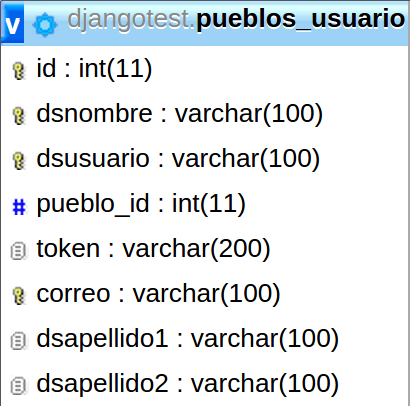
\includegraphics[scale=0.25]{./django/imagenes/tabla.png}
\caption{Tabla Usuarios de la base de datos Semandal}
\label{tablausuario}
\end{figure}

A continuación explicaremos los tipos de datos, que hemos usado en nuestro models, se pueden asignar con django y las opciones de éstas.
\begin{description}
  	\item[CharField] \hfill \\
  		Éste método crea un atributo de tipo Texto
  	\item[BooleanField] \hfill \\
  		Crea un atributo de tipo boolean, 
  	\item[PositiveIntegerField] \hfill \\
  		Crea un entero mayor que cero.
  	\item[DateTimeField] \hfill \\
  		Crea un atributo de tipo fecha.
\end{description}
\subsection{Manejo de la base de datos con django}

En esta sección realizaremos una enumeración de los comandos importantes en django, que hemos utilizado para nuestro proyecto.

\subsection{Creación de registro en una tabla}

Para crear un nuevo registro en la tabla, en primer lugar debemos crear el objeto. Si en el models, no hemos especificado que un campo puede ser null debemos agregarlo obligatoriamente, en caso contrario al intentar insertarlo django nos dará error.

\begin{lstlisting}
		sigp = SigP(id_user=u,id_p=p[0])
\end{lstlisting}

Cabe recordar que si la tabla tenía una clave foránea, como es el caso de nuestro ejemplo, \textit{u} y \textit{p[0]} deben ser objetos de tipo usuario y pueblo respectivamente por tanto debemos o crearlos antes o extraerlos de una consulta

\subsection{Consulta de un registro en una tabla}

Antes que nada, en las consultas de los registros explicamos que, cuando se iban a buscar objetos que tenían claves foraneas, debíamos pasar en la busqueda el objeto o una referencia. En el siguiente ejemplo, en la primera linea pasamos objetos, y en la segunda, decimos que de la tabla SigP, el objeto usuario tiene un id = u\_id.

		\begin{lstlisting}
			sigue = SigP.objects.filter(usuario=u,pueblo = p)
			sigue = SigP.objects.filter(usuario__id=u_id,pueblo__id = p_id)
		\end{lstlisting}

De manera general, sería algo parecido a:

		\begin{lstlisting}
			sigue = tabla1.objects.filter(atributo(tabla1)=Objeto)
			sigue = tabla1.objects.filter(atributo(tabla1)__atributo(tabla2)=Atributo(tabla2))
		\end{lstlisting}

En el proyecto usamos las dos, para demostrar que funciona de cualquier manera, pero la manera más correcta sería la segunda.

Vamos a explicar a continuación las dos maneras que existen de consultar registros de una tabla con django.
\begin{description}
  \item[filter] \hfill \\
  	Filter se trae un QuerySet. Es decir, una lista de objetos de la tabla que consultemos. Si la consulta no devuelve ningún valor nos devolverá una lista vacía.
	\begin{lstlisting}
		sigue = SigP.objects.filter(usuario=u,pueblo = p)
	\end{lstlisting}
	

  \item[get] \hfill \\
  Lo que nos devuelve get es un único objeto de tipo SigP (En este caso). De hecho, si intentamos realizar el \textit{\"Where\"} y esa consulta nos da más de un resultado, django nos dará un error.
	\begin{lstlisting}
		SigP.objects.get(id=x)
	\end{lstlisting}
\end{description}

También tienen conversión los operandos clásicos de ayuda en las búsquedas

\begin{description}
	\item[order\_by] \hfill \\
	 Éste quizas sea el operador que tiene la sintaxis más simple de todos los operadores auxiliares de búsqueda. Simplemente debemos escribir el \textbf{Order\_By()} y entre los paréntesis el campo por el que queremos ordenar. 
	\begin{lstlisting}
		rez = Comentarios.objects.filter(id_not=n_id).order_by('fecha')	
	\end{lstlisting}
	
	\item[reverse] \hfill \\
	 Este operador es el ASC o DSC del SQL clásico. Por defecto el order by los ordena ascendentemente y el reverser le da la vuelta al resultado de la consulta.
	 
	 \item[distinct]\hfill \\
	 Este es uno de los más complicados ya que tienen dos formas de invocarlo y dos resultados distintos.
	 \begin{description}
	  \item[values]
	  	Nos devuelve un diccionario. A continuación pondremos una consulta y una imagen con el resultado que devuelve.
	  \begin{lstlisting}
	 	Noticias.objects.order_by().values('id').distinct()  
	  \end{lstlisting}
	\begin{figure}[h]
	  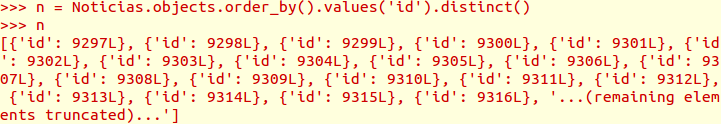
\includegraphics[width=\textwidth]{./django/imagenes/values.png} 
	\caption{Diccionario devuelto}
	\end{figure}	   

	  \item[values\_list]
	  	Este método devuelve una lista de tuplas. 
	  \begin{lstlisting}
	 	Noticias.objects.order_by().values_list('id').distinct()  
	  \end{lstlisting}
	\begin{figure}[h]
	  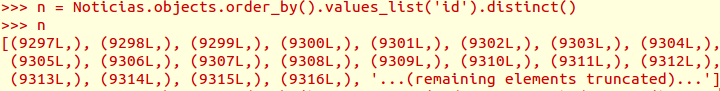
\includegraphics[width=\textwidth]{./django/imagenes/values_list.png} 
	\caption{Lista de Tuplas de valores devueltos}
	\end{figure}	   

	  También podemos agregar en la consulta de values el parámetro flat a True, para que este nos devuelva una lista.
	  \begin{lstlisting}
	 	Noticias.objects.order_by().values_list('id',flat=True).distinct()  
	  \end{lstlisting}
	\begin{figure}[h]
		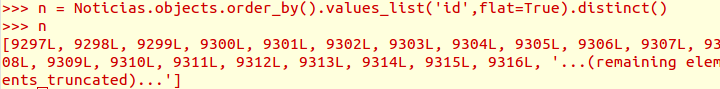
\includegraphics[width=\textwidth]{./django/imagenes/distinct_list.png}
	\caption{Lista de valores devueltos}
	\end{figure}	   

	\end{description}

\end{description}

\subsection{Actualizar registro en django.}

El método update de django se realiza sobre un QuerySet, por tanto debemos realizar un filter para obtener el objeto en el queryset que queremos y posteriormente escribir el siguiente comando

	  \begin{lstlisting}
		Objeto.update(Atributo = NuevoValor)
	  \end{lstlisting}



\subsection{Mysql con django}

	Django es un entorno de programación que da un paso más en cuanto al manejo de la base de datos. Django lo que hace es estar en un punto intermedio entre las bases de datos clásicas y las bases de datos orientadas a objetos. Desde el punto de vista del programador las consultas ya no se hacen de forma clasica, si no que debemos trabajar con objetos.
	Cuando realizamos una consulta, lo que django nos devuelve es un array de objetos. Y cuando trabajamos con claves foráneas, en el manejo de bases de datos clásico, hacíamos un inner join y consultábamos el id de la tabla que necesitábamos en el where. Con el manejo de bases de datos con objetos, debemos o consultar el objeto que tiene una series de características y después pasarlo en otra búsqueda, o hacer una referencia en la búsqueda. A continuación realizaremos un ejemplo del empleo de ambas consultas.
	
	\begin{enumerate}
	
		\item Busqueda de un objeto referenciando el objeto a buscar en la busqueda
		\begin{lstlisting}
			pueblos = SigP.objects.filter(id_user__id = id_u).order_by("id_p__dspueblo")
		\end{lstlisting}
		\item Busqueda de un objeto buscando el objeto que referenciaba antes
			\begin{lstlisting}
			usuario = Usuario.objects.filter(id=id_u)[0]
			pueblo = Pueblo.objects.filter(id=id_p)[0]
			u = SigP(id_user=usuario,id_p=pueblo)
		\end{lstlisting}
	\end{enumerate}
	
Este apartado quizás sea uno de los más extensos porque 

	En django, las direcciones accesibles se expresan en un fichero (urls) y se definen estas con una expresión regular. Si una dirección a la que intentan acceder a nuestro servidor django no cumple una de las expresiones regulares que tenemos definidas en el urls.py, nos saltará una excepción en el navegador. Además de la expresión regular, el código que se ejecuta en nuestro servidor web es un método definido y desarrollado en el views.py el cual explicaremos a continuación.
	
	En definitiva el urls.py, es como el funcionamiento de un \textit{switch-case}. Si la url cumple una expresión regular, ejecuta el método en el views.py que esté especificado en la misma linea.
	
\begin{lstlisting}
    url(r\'\textasciicircum RegularExpresion/$\', views.metodo, name=\'metodo\')
\end{lstlisting}	

\section{Ejecución de código - /polls/views.py}
	
	Este realmente es nuestro quid de la cuestión. Cada método escrito en el views.py debe devolver un HttpRespone(). 
	esta respuesta http, puede ser escrita en un fichero html a parte o bien (Nosotros únicamente queremos respuestas json para nuestra aplicación) enviar en una respuesta http, una cadena de texto en formato json.
	Al estar todo basado en un lenguaje de programación (Python) podemos usar los métodos de python para transformar las respuestas en json o bien podemos parsear nosotros el propio json para obtener lo que queremos en éste. 
	La última opción será por la que nos decantemos ya que por defecto nos da los datos y nombres de una consulta y nosotros queremos únicamente ciertos datos para no sobrecargar la respuesta json.
	También podemos pasar parámetros a estos métodos por la url, especifícandolos en la expresión regular de urls.py.
	
\section{Definición de parámetros en el proyecto - /mysite/settings.py}
	
En este fichero, tenemos los atributos del proyecto. A continuación pondremos los atributos más importantes pero no todos los qeu están especificados.

\begin{description}

	\item[INSTALLED APPS]
		Esta son las APIS que usan nuestra aplicación, debemos especificar aquí todas aquellas que vamos a crear. Por defecto vienen especificadas algunas aplicaciones nativas de django como la de administrador o la de autentificación.
	\item[DATE\_INPUT\_FORMATS]
		Como su propio nombre indica, muestra como se manejarán las fechas y con qué formatos, en nuestro proyecto
	\item[SECRET\_KEY]
		Usado para la codificación a la hora de entrar en la aplicación, loguearse como usuario, por ello, debe ser un valor no predecible y único. También es creado de forma automática aunque podemos cambiarlo.
	\item[LANGUAGE\_CODE]
		El idioma que vamos a usar para nuestra aplicación.
	\item[TIME\_ZONE]
		La zona horaria que usaremos para obtener fechas.
	\item[DATABASES]
		Las bases de datos que usaremos en nuestro proyecto. En éste debemos especificar el motor, el nombre de la tabla, el nombre de usuario y su contraseña y por último, la dirección. 
		\begin{lstlisting}
DATABASES = {
    'default': {
        'ENGINE': 'django.db.backends.mysql',
        'NAME': 'tabla',
		'USER':'user',
		'PASSWORD':'userpass',
		'HOST':'host.uhu.es',
    }
}		
		\end{lstlisting}
		\end{description}

%%PARTE EXTRA

\section{Creación de comandos personalizados}

La ejecución de scripts en Django se realiza a través de la shell ejecutando el ficheto manager.py. Para la ejecución de tareas periódicas se recomienda la creación de comandos para facilitar la ejecución automática de las tareas. Para la creación de los comandos se debe modificar la estructura de archivos creada durante la instalación de Django, para permitir la ejecución de comandos personalizados se debe modificar la estructura de la siguiente manera:

\begin{lstlisting}
polls/
    __init__.py
    models.py
    management/
        __init__.py
        commands/
            __init__.py
            _private.py
            closepoll.py
    tests.py
    views.py
\end{lstlisting}

Siguiendo el ejemplo de la creación de la aplicación polls, la modificación incluye la creación de los ficheros \textit{management} y \textit{commands}. Dentro de esta última carpeta se incluyen los ficheros con el código que se ejecutará con el comando, el nombre del comando es el mismo que se le de al fichero. Si el nombre del fichero comienza con guión bajo (\_) el comando no se podrá ejecutar.

El código que incluye el fichero que contiene el código del comando es el siguiente:

\begin{lstlisting}
import sys
sys.path.insert(0, '...django/mysite/Programas/Update/')
import mi_modulo
from django.core.management.base import NoArgsCommand

class Command(NoArgsCommand):
    def handle_noargs(self, **options):
		mi_modulo.run()

\end{lstlisting}

Con este código se crea un comando sin argumentos. Con el módulo sys se agrega a la variable PATH de Python la ruta al script que realiza la extracción de noticias, de esta forma luego podemos exportarlo como un módulo y ejecutarlo.

Para ejecutar el comando, lo utilizamos como argumento al ejecutar el fichero manage.py


\begin{lstlisting}
python ./manage.py mi_comando
\end{lstlisting}
\section{Uso de Django-extensions}
Django-extension es un conjunto de comandos y extras que se añaden a la funcionalidad que ofrece Django. Una vez instaladas las extensiones, hay que agregarlas a la aplicación que se está creando. Para agregarla hay que modificar la variable INSTALLED\_APPS que se encuentra en el fichero \textit{settings.py}:

\begin{lstlisting}
INSTALLED_APPS = (
    ...
    'django_extensions',
)
\end{lstlisting}

Una vez instalado, puede generarse el fichero dot que contiene un grafo creado a partir del modelo creado en django con el siguiente comando:

\begin{lstlisting}
manage.py graph_models -a > my_project.dot
\end{lstlisting}

Con el fichero dot podemos obtener el grafo en formato PNG con el siguiente comando:

\begin{lstlisting}
dot -Tpng my_project.dot > my_project.png
\end{lstlisting}

\section{Anotaciones}
	
Cuando investigamos no sabemos a priori los datos que vamos a necesitar de un objeto (Municipio en nuestro caso), y por tanto a medida que van surgiendo nos encontramos con que debemos modificar la tabla. Para esto hay un plugin llamado \textit{South} cuya función consistía en migrar la base de datos. Esta opción quedó descartada debido a la gran cantidad de datos así que se optó por agregar el campo al models y de la misma forma agregarlo a partir de la herramienta de MySQL \textit{PHPMyAdmin} ya que los cambios se iban haciendo para un campo o dos, pero al final recurrimos muy a menudo a esta solución ya que la mayoría de cambios se hicieron en la tabla de pueblo y esta tabla no era conveniente borrarla ya que los datos no eran reproducibles en un corto plazo debido a que algunos de los campos eran rellenados a partir de datos buscados con un script que usaba la API de búsqueda de google como hemos referenciado en este capitulo.
	Otra solución para este problema que se nos presentaba era borrar la tabla (Si no tenía este tipo de datos y volver a llamar al comando syncdb.
	Otra herramienta muy potente de django que no hemos usado es \textit{TastyPie}. Esta herramienta es la que nos ayudaba en la creación de la RestAPI. Pero decidimos no usarla por la descentralización y poder devolver los errores de la forma que queríamos. En los estudios realizados sobre esta herramienta no hemos visto la posibilidad de realizar estas acciones y se hicieron varias pruebas de decodificación de los datos que nos devolvía la \textit{API} con \textit{TastyPie} y el método de codificación que nos daba \textit{Python}, y no funcionaron correctamente por lo que decidimos realizar nosotros la conversión en \textit{JSON}

Por último una de las cosas más importantes a la hora de la preparación de los datos es la paginación. Es una funcionalidad que agregamos al proyecto una vez que éste estaba con las funcionalidades básicas implementadas y con un correcto funcionamiento. Posteriormente nos dedicamos a pulir las funcionalidades y una muy importante era ésta. No debíamos traernos por ejemplo todas las noticias ya que esto hacía que la aplicación tardara mucho a la hora de realizar esta consulta porque el pueblo que más noticias tiene son 3800. Entonces teníamos que diseñar el sistema de paginación y trabajar con el. Al principio creamos uno manual en el que le íbamos indicando de qué a qué noticia me traía, pero si un futuro queremos poner publicidad en nuestra API en la página web, y la gente puede entrar y traerse toda la información, no tendrá muchas visitas. Del mismo modo, tenemos información que hemos recopilado y tratado. Este proceso nos ha llevado mucho tiempo, y si un usuario puede obtener todos los datos de la base de datos en un sólo click sería contraproducente para nosotros ya que todo nuestro trabajo se podría copiar con mucha facilidad.
%%%%%%%%%%%%%

